\section{Correctness\label{section:inductive-correctness}}

This section provides correctness arguments and proofs for the different settings of our inductive approach to state machine synthesis. The simplest approach with RPNI is first discussed; features are then gradually integrated, such as scenario questions and the injection of domain knowledge. A deeper analysis of the problem statement and an overview of this section is first given in Section~\ref{section:inductive-correctness-overview}.

\subsection{Overview\label{section:inductive-correctness-overview}}

In view of the initial problem statement in Section~\ref{subsection:inductive-synthesis-statement} and its successive strengthening in subsequent sections, proving the correctness of our approach amounts to show that the composed system resulting from synthesis is consistent with input scenarios and all injected domain knowledge. 

\begin{figure}\centering
\scalebox{.65}{
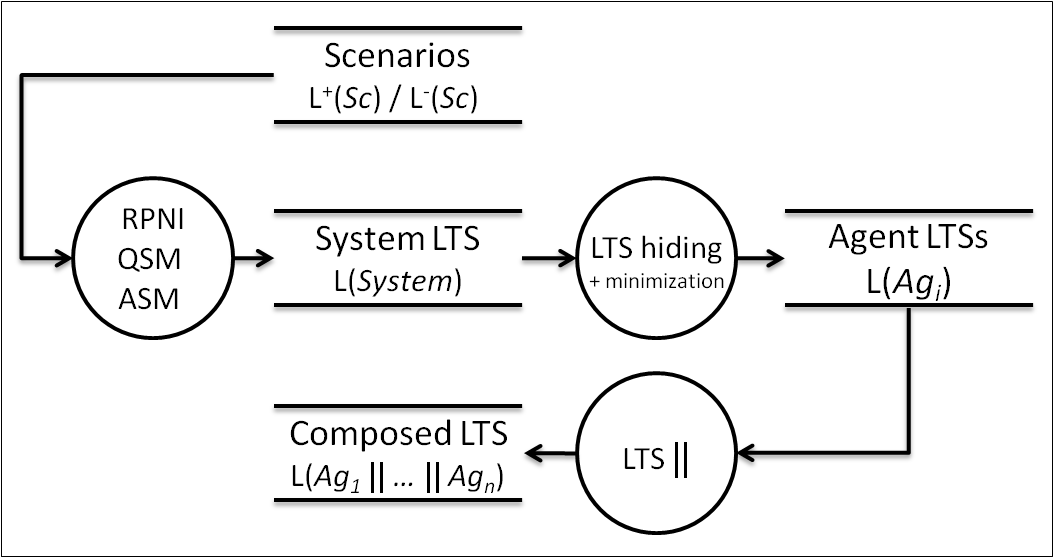
\includegraphics[trim=3mm 3mm 3mm 3mm, clip]{src/4-inductive/images/synthesis-flow-model}}
\caption{Inductive synthesis steps and products.\label{figure:synthesis-flow-model}} 
\end{figure}

Fig.~\ref{figure:synthesis-flow-model} summarizes our synthesis approach. It shows the algorithms used together with their input/output in terms of behavior models and associated languages. Such figure can be read as follows:
\begin{itemize}
\item From scenarios, a system LTS is inferred using RPNI, QSM or ASM. 
\item LTS hiding and minimization is then used to obtain a canonical state machine for each agent. 
\item From the system view point, the result of our synthesis approach is precisely captured by the composition of those state machines.
\end{itemize}

In this figure and in the following discussions,
\begin{itemize}
\item $Sc = (S^+,S^-)$ denotes the input scenario collection; its positive and negative languages are denoted by $\mathcal{L}^+(Sc)$ and $\mathcal{L}^-(Sc)$, respectively. 

When considering ASM, $Sc$ denotes both the input hMSC and the scenario collection (see Section~\ref{section:inductive-from-hMSC}). The positive and negative languages are updated accordingly. 
\item $\mathcal{L}(\me{System})$ denotes the language captured by the inferred system LTS.
\item $\mathcal{L}(Ag)$ denotes the language of an arbitrary agent $Ag$, as captured by its LTS state machine.
\item $\mathcal{L}(\agentscomposed)$ denotes the language captured by the LTS resulting of the composition of the individual agent LTSs.
\end{itemize}

Remember from Section~\ref{subsection:inductive-synthesis-statement} that, under the precondition that input models are consistent, three conditions are required to hold on the synthesized state machines:
\begin{itemize}
\item The \emph{structural consistency} condition requires input scenarios and synthesized agent state machines to agree on the respective agent interfaces. 

In the case of QSM, structural consistency must also hold for answers to scenario questions. In the case of ASM, this applied to the input hMSC as well.

\item The \emph{consistent agent view} condition requires each synthesized agent state machine to cover the positive behaviors along the corresponding scenario timeline.
\begin{align}
\mathcal{L}^+(Sc_{\downarrow Ag}) \subseteq \mathcal{L}(Ag)\mbox{~for each agent $Ag$}\label{proof:consistent-agent-view}
\end{align}
where $Sc_{\downarrow Ag}$ denotes the positive behaviors along $Ag$'s timeline in a scenario collection $Sc = (S^+, S^-)$:
\begin{align}
\mathcal{L}^+(Sc_{\downarrow Ag}) = \bigcup_{P \in S^+} \mathcal{L}(P_{\downarrow Ag})~\cup~\bigcup_{N \in S^{-}} \mathcal{L}^{+}(N_{\downarrow Ag})\label{proof:lemma-sc-projection}
\end{align}

This is a a slight generalization of the concept of agent traces along the timeline of a single scenario, see $M_{\downarrow Ag}$ in Section~\ref{section:background-scenarios}. Observe that $\mathcal{L}^+(Sc_{\downarrow Ag})$ takes both positive and negative scenarios into account.

In the case of QSM, (\ref{proof:consistent-agent-view}) must hold even when $Sc$ is assumed to contain the answers to scenario questions. In the case of ASM, (\ref{proof:consistent-agent-view}) remains the same, but the projection of the input hMSC $H$ has to be considered in addition to the scenario collection in (\ref{proof:lemma-sc-projection}):
\begin{align}
\mathcal{L}^+(Sc_{\downarrow Ag}) = \bigcup_{P \in S^+} \mathcal{L}(P_{\downarrow Ag})~\cup~\bigcup_{N \in S^{-}} \mathcal{L}^{+}(N_{\downarrow Ag})~\cup~\mathcal{L}(H_{\downarrow Ag})\label{proof:lemma-sc-projection-asm}
\end{align}

\item The \emph{consistent system view} requires the composed system to cover all positive scenarios and reject all negative ones. 
\begin{align}
&\mathcal{L}^+(Sc) \subseteq \mathcal{L}(\agentscomposed)\label{proof:consistent-system-view-1}\\
&\mathcal{L}^-(Sc) \cap      \mathcal{L}(\agentscomposed) = \emptyset\label{proof:consistent-system-view-2}
\end{align}

In the case of QSM, $Sc$ is assumed to contain answers to scenario questions. In the case of ASM, $Sc$ denote the input hMSC together with the scenario collection.

When goals are injected in the induction process, this postcondition must be strengthened with the following condition requiring the goals to be rejected by the synthesized system:
\begin{align}
&\mathcal{L}^-(\me{Goals}) \cap      \mathcal{L}(\agentscomposed) = \emptyset
\end{align}
where $\mathcal{L}^-(\me{Goals})$ denotes the union of all system traces violating at least one known goal.
\begin{align}
&\mathcal{L}^-(\me{Goals}) = \mathcal{L}^-(G_1) \cup \ldots \cup \mathcal{L}^-(G_n)
\end{align}

\end{itemize}

The following sections are organized as follows. Section~\ref{subsection:system-lts-consistency} establishes a first milestone by proving the consistency of the inferred system LTS with scenarios in the case of RPNI. This result is then used in Section~\ref{subsection:consistent-agent-view} to show that the decomposition step meets the ``structural consistency'' and the ``consistent agent view'' conditions. The ``consistent system view'' condition is further discussed in Section~\ref{subsection:consistent-system-view}. The discussion is pursued in the presence of scenario questions in Section~\ref{subsection:proof-with-scenario-questions} and with the injection of goals in Section~\ref{subsection:proof-with-domain-knowledge}. Section~\ref{subsection:correctness-of-asm} closes this section by discussing the correctness of ASM.

%%%

\subsection{Consistency of the system LTS\label{subsection:system-lts-consistency}}

This section demonstrates that RPNI yields a system LTS consistent with the input scenario collection. The pseudo code given in Algo.~\ref{QSM} is used; the inner-most while loop related to scenario questions is ignored here (lines 5 to 10).

\begin{theorem}
\label{theorem:system-lts-consistency-with-sc}
The system LTS synthesized by RPNI covers all positive scenarios and rejects all negative ones.
\begin{align*}
&\mathcal{L}^+(Sc) \subseteq \mathcal{L}(System)\\
&\mathcal{L}^-(Sc) \cap      \mathcal{L}(System) = \emptyset
\end{align*}

\begin{proof}
This theorem is proven by induction using the following invariant:
\begin{align}
&\mathcal{L}^+(Sc) \subseteq \mathcal{L}(A_i)\label{inv:system-lts-consistency-with-sc-1}\\
&\mathcal{L}^-(Sc) \cap      \mathcal{L}(A_i) = \emptyset\label{inv:system-lts-consistency-with-sc-2}
\end{align}

\begin{description}
\item[Base:] $A_0$ denotes the PTA returned by \emph{Initialize}.

The PTA is the largest DFA accepting exactly the positive language; an algorithm precondition also states that input scenarios are consistent. Therefore the following conditions hold, entailing the invariant:
\begin{align*}
&\mathcal{L}^+(Sc) =    \mathcal{L}(A_0)\\
&\mathcal{L}^-(Sc) \cap \mathcal{L}(A_0) = \emptyset
\end{align*}

\item[Inductive step:] $A_i$ is the quotient automaton denoting the current solution at step $i$; (\ref{inv:system-lts-consistency-with-sc-1}) and (\ref{inv:system-lts-consistency-with-sc-2}) are assumed to hold on the candidate automaton $A_i$.

From a solution $A_i$, the next solution $A_{i+1}$ is computed by the \emph{Merge} function (see line 3 in Algo.~\ref{QSM}). The latter computes a quotient automaton of $A_i$. We prove the positive and negative parts of the invariant in turn.

On one hand, Definition~\ref{definition:quotient-automaton} guarantees that such quotient automaton may only generalize the language of $A_i$. As the condition~(\ref{inv:system-lts-consistency-with-sc-1}) is assumed to hold for $A_i$, the following condition holds as well:
\begin{align*}
&\mathcal{L}^+(Sc) \subseteq \mathcal{L}(A_i) \subseteq \mathcal{L}(A_{i+1})
\end{align*}

On the other hand, a candidate solution is only kept for the next iteration if it is consistent with the negative scenarios (see lines 4 and 11). Therefore, the following condition holds when such solution is kept (line 11):
\begin{align*}
&\mathcal{L}^-(Sc) \cap \mathcal{L}(A_{i+1}) = \emptyset
\end{align*}

When the algorithm terminates, it returns the last compatible quotient automaton considered.
\end{description}
\end{proof}
\end{theorem}

A detailed proof of the convergence of RPNI towards the canonical target automaton when it receives a characteristic sample can be found in~\cite{Oncina:1993} in the more general case of transducer learning.

%%%

\subsection{Structural consistency and consistent agent view\label{subsection:consistent-agent-view}}

Given the consistency of the system LTS with the positive and negative scenarios, the decomposition step guarantees that the \emph{structural consistency} and the \emph{consistent agent view} both hold. We only sketch the structure of such proofs here. 

Structural consistency only requires the LTS hiding step to make use of adequate agent alphabets, as induced from the scenarios themselves or given by a (consistent) structural model. We do not discuss it further. 

For each agent $Ag$, the ``consistent agent view'' condition (\ref{proof:consistent-agent-view}) is derived from (\ref{proof:consistent-system-view-1}) using the following derivations:
\begin{align}
&\mathcal{L}(X) \subseteq \mathcal{L}(Y) \implies \mathcal{L}(X \setminus I) \subseteq \mathcal{L}(Y \setminus I) \label{proof-agent-consistency-1}\\
&\mathcal{L}^+(Sc_{\downarrow Ag}) = \mathcal{L}^+(Sc \setminus \Sigma_{Ag}^c)\label{proof-agent-consistency-2}\\
&\mathcal{L}(Ag) = \mathcal{L}(System \setminus \Sigma_{Ag}^c)\label{proof-agent-consistency-3}
\end{align}
where $\Sigma_{Ag}^c$ denotes the set of all system events excluding those of $Ag$'s interface.
\begin{itemize}
\item (\ref{proof-agent-consistency-1}) states that behavior inclusion is preserved under LTS hiding; this property follows from material in Section~\ref{subsection:lts-hiding}. 
\item (\ref{proof-agent-consistency-2}) rewrites the left term of (\ref{proof:consistent-agent-view}) in terms of the hiding of scenario behaviors\footnote{using an abuse of notation here as the hiding operator is defined on LTS, not on scenarios collections.}. For RPNI and QSM, it can be derived from (\ref{proof:lemma-sc-projection}) and the definition of $M_{\downarrow Ag}$ (see Section~\ref{subsection:background-positive-scenarios}). For ASM, it can be derived in a similar way from (\ref{proof:lemma-sc-projection-asm}).
\item (\ref{proof-agent-consistency-3}) follows from the definition of the decomposition step itself (see (\ref{definition:decomposition-step}) in Section~\ref{subsection:inductive-synthesis-approach}). 
\end{itemize}

Theorem~\ref{theorem:system-lts-consistency-with-sc} establishing the consistency of the system LTS with input scenarios, the following condition is established thanks to (\ref{proof-agent-consistency-1})
\begin{align}
&\mathcal{L}^+(Sc \setminus \Sigma_{Ag}^c) \subseteq \mathcal{L}(System \setminus \Sigma_{Ag}^c)\label{proof:consistent-agent-view-milestone}
\end{align}

The ``consistent agent view'' condition (\ref{proof:consistent-agent-view}) is established by substituing the right terms of (\ref{proof-agent-consistency-2}) and (\ref{proof-agent-consistency-3}) in (\ref{proof:consistent-agent-view-milestone}).

%%%

\subsection{Consistent system view: the problem of implied scenarios\label{subsection:consistent-system-view}}

This section discusses the correctness of the ``consistent system view'' condition in the case of RPNI. The conditions related to the positive and negative scenarios are discussed in turn.

\begin{theorem}
When using the RPNI induction algorithm, the composed system synthesized by the inductive approach covers all positive scenarios.
\begin{align*}
&\mathcal{L}^+(Sc) \subseteq \mathcal{L}(\agentscomposed)
\end{align*}

\begin{proof}
This condition results from two main properties:
\begin{itemize}
\item Theorem~\ref{theorem:system-lts-consistency-with-sc} establishing the consistency of the inferred system LTS.
\begin{align*}
&\mathcal{L}^+(Sc) \subseteq \mathcal{L}(System)
\end{align*}
\item Projecting the system LTS on agent alphabets and recomposing their LTS afterwards does not restrict behaviors:
\begin{align*}
&\mathcal{L}(\mbox{System}) \subseteq \mathcal{L}(\agentscomposed)
\end{align*}
This latter condition can be derived from the definition of agent languages (\ref{proof-agent-consistency-3}) and properties of LTS hiding and composition operators (see Section~\ref{section:background-state-machines}).
\end{itemize} 

\end{proof}
\end{theorem}

\begin{theorem}[Candidate]
When using the RPNI induction algorithm, the composed system synthesized by the inductive approach rejects all negative scenarios.\label{theorem:consistent-system-view-negative}
\begin{align*}
&\mathcal{L}^-(Sc) \cap \mathcal{L}(\agentscomposed) = \emptyset
\end{align*}
\end{theorem}

Due to the potential presence of implied scenarios, our approach only guarantees the weaker postcondition already given by Theorem~\ref{theorem:system-lts-consistency-with-sc}, namely,
\begin{align*}
&\mathcal{L}^-(Sc) \cap \mathcal{L}(\mbox{System}) = \emptyset
\end{align*}

In other words, the induction algorithm ensures that the system LTS excludes all negative scenarios. This property can however be lost after the decomposition and recomposition steps leading to the composed system.

The reason has to be found in the possible occurence of so-called \emph{implied scenarios} \cite{Alur:2000, Uchitel:2004}. Remember from Section~\ref{subsection:background-hmsc} that implied scenarios may appear when a system is specified system-wide while implemented component-wise. 

In our case, the set of implied scenarios is precisely defined as:
\begin{align}
\mathcal{L}(\agentscomposed) \setminus \mathcal{L}(\mbox{System})\label{proof:set-of-implied-scenarios}
\end{align}
that is, implied scenarios denote system behaviors that the system LTS does not accept but which are exhibited by the composition of agent LTSs. Implied scenarios appear when, once distributed, the agents lack monitoring and controlling abilities to restrict their behavior so as to precisely match the system LTS.

Three cases may arise here:
\begin{itemize}
\item The set of implied scenarios (\ref{proof:set-of-implied-scenarios}) is empty. 

In this case, the inferred system LTS and the composed system coincide. Therefore, Theorem~\ref{theorem:consistent-system-view-negative} is a trival consequence of Theorem~\ref{theorem:system-lts-consistency-with-sc}.

\item The set of implied scenarios (\ref{proof:set-of-implied-scenarios}) only contains examples of desired system behaviors.

Theorem~\ref{theorem:consistent-system-view-negative} is trivially proven as implied scenarios do not intersect with negative scenarios. 

In this case, the presence of implied scenarios is not problematic and may be seen as the result of a second generalization step due to the decomposition and recomposition of agent LTS. This second generalization step proves useful as it weakens the necessity of having a pure structurally complete scenario collection in the first place.

\item The set of implied scenarios (\ref{proof:set-of-implied-scenarios}) contains at least one counterexample of desired system behaviors. 

This case is more problematic. In particular, a behavior trace $t$ could be such that the following conditions hold:
\begin{align}
&t \in \mathcal{L}^-(Sc)\label{implied-1}\\
&t \notin \mathcal{L}(\mbox{System})\label{implied-2}\\
&t \in \mathcal{L}(\agentscomposed)\label{implied-3}
\end{align}
that is, (\ref{implied-1}) $t$ denotes a system behavior explicitly rejected through a negative scenario; it might be a question answered negatively; (\ref{implied-2}) $t$ is correctly rejected by the system LTS; (\ref{implied-3}) $t$ is still be exhibited by the composed system.

In such case, the candidate Theorem~\ref{theorem:consistent-system-view-negative} is shown too strong.  The ``consistent system view'' condition is not met as (\ref{proof:consistent-system-view-2}) does not hold. As with other scenario approaches, e.g. \cite{Alur:2000, Uchitel:2004}, our synthesis technique fails to guarantee a consistent system view between scenarios and state machines in presence of negative implied scenarios.

In order to detect such situations, the technique from \cite{Uchitel:2004} could be adapted to enumerate implied scenarios and submit them as additional scenario questions to the user (see Section~\ref{section:related-for-analysis-3}). 

Note that, fixing implied scenario problems requires rethinking the system decomposition into agents and/or refactoring their interfaces. In other words, the root cause of implied scenarios problems has to be found in the structural decomposition of the system, not in the particular technique used to infer state machines from scenarios. 

\end{itemize}

%%%

\subsection{Correctness in the presence of scenario questions\label{subsection:proof-with-scenario-questions}}

The postcondition of our approach was strengthened in the presence of scenario questions. This strengthening required the synthesized system to be consistent with all scenario questions in addition to the initial scenario collection. 

Provided a consistent system LTS is inferred with QSM, the correctness arguments for the \emph{structural consistency} and \emph{consistent agent view} conditions remain unchanged. The discussion about implied scenarios also takes place here. Therefore, we only prove the consistency of the system LTS induced by QSM when scenario questions are taken into account.

\begin{theorem}
The system LTS inferred by QSM is consistent with the scenario collection extended with the answers to all scenario questions.

\begin{proof}
This theorem is proven by induction (cfr. Algo.~\ref{QSM}):
\begin{description}
\item[Base:] The base case captures a QSM run where all scenario questions are answered positively. 

In such case, QSM roughly reduces to RPNI, for which Theorem~\ref{theorem:system-lts-consistency-with-sc} is known to hold. We still need to prove that all scenario questions are accepted by the synthesized system LTS. 

Observe that all scenarios accepted at line 7 are consistent with the current solution $A_{new}$ (line 4). The system LTS returned by QSM is a quotient automaton of $A_{new}$; Definition \ref{definition:quotient-automaton} therefore ensures that the system LTS accepts those scenarios as well.

\item[Inductive step:] The inductive step captures a run where a rejected scenario yields a tail recursive call (line 10).

The discussion about positively accepted scenarios remains unchanged. The scenario collection is correctly extended (see line 7).

Every time a scenario question is rejected by the oracle, the scenario collection is correctly extended as well (see line 9). Provided the oracle does not make classification errors, as required in preconditions, the scenario collection remains consistent for the tail recursive call taking place at line 10.
\end{description}
\end{proof}
\end{theorem}

%%%

\subsection{Consistency with goals and domain properties\label{subsection:proof-with-domain-knowledge}}

The pre- and postconditions of our approach were strenghtened in the presence of goals and domain properties. In precondition, scenarios and goals are required to be consistent. In postcondition, the synthesized system may not violate goals. In other words, provided the input scenarios and safety properties are consistent, the following postcondition is required to hold:
\begin{align}
&\mathcal{L}^-(\me{Goals}) \cap \mathcal{L}(\agentscomposed) = \emptyset \label{consistency-of-system-lts-with-goals}
\end{align}

A weaker condition is proven in Theorem~\ref{theorem:system-lts-consistency-with-goals} as implied scenarios may lead to goals being violated after the decomposition and recomposition steps. A few simplicifcations are in order here:
\begin{itemize}
\item We consider here the case of RPNI; in the absence of classification errors by the oracle, the injection of goals is independent of the scenario questions. 
\item In accordance with the assumptions of the thesis we consider only safety properties (see \ref{section:background-goals}).
\item Without lost of generality, we consider only one of such safety properties, $G$. 
\end{itemize}

Lemma~\ref{lemma:qsm-and-tester-prefixes} provides a useful milestone.

\begin{lemma}
When two states $q$ and $q'$ are considered for merging by QSM, all their prefixes are traces leading to the same state in the tester automaton capturing $\mathcal{L}^-(G)$.\label{lemma:qsm-and-tester-prefixes}
\begin{proof}
We assume the correctness of the joint traversal for annotating the PTA states with their corresponding states in the tester automaton (see Section~\ref{subsection:induction-pruning-with-goals}). The induction algorithm will only consider the merging of state pairs corresponding to the same state in the tester automaton. The prefixes property thus holds for the first merge considered on the PTA; it is trivially preserved under state merging and therefore holds for every state pair considered from the successive quotient automata.
\end{proof}
\end{lemma}

\begin{theorem}
\label{theorem:system-lts-consistency-with-goals}
Provided $G$ denotes a safety property, the system LTS synthesized by the constrained inductive algorithm is consistent with $G$.
\begin{align*}
&\mathcal{L}^-(G) \cap \mathcal{L}(\emph{System}) = \emptyset
\end{align*}

\begin{proof}
The proof proceeds by induction on the following loop invariant:
\begin{align*}
\mathcal{L}^-(G) \cap \mathcal{L}(A_i) = \emptyset
\end{align*}

\begin{description}
\item[Base:] $A_0$ denotes the PTA.

The invariant holds for $A_0$ as (1) the preconditions require the scenarios and the goals to be consistent and (2) the PTA does not generalize the positive scenario language.
\begin{align*}
&\mathcal{L}^-(G) \cap \mathcal{L}^+(Sc) = \emptyset\\
&\mathcal{L}(A_0) = \mathcal{L}^+(Sc)
\end{align*}

\item[Inductive step:] Let $A_i$ denote a current solution considered by the algorithm. Suppose the invariant holds for $A_i$. We show that the invariant holds for $A_{i+1}$, the quotient automaton of $A_i$ obtained by merging a candidate state pair $(q,q')$.

By construction of the constraint mechanism based on equivalent state classes, $q$ and $q'$ correspond to the same state $t$ in the tester automaton capturing $\mathcal{L}^-(G)$ (see Section~\ref{subsection:induction-pruning-with-goals}).

The tester is known to be a canonical automaton, that is, it is minimal and deterministic (see Section~\ref{subsection:background-property-and-tester-automata}). A bijection thus exists between states and accepted trace suffixes (residual languages)~\cite{Hopcroft:1979}. 

Therefore, all accepted traces from $q$ (resp. $q'$) in the current solution $A_i$ are rejected traces from $t$ in the tester automaton. By Lemma~\ref{lemma:qsm-and-tester-prefixes} all prefixes of $q$ in $A_i$ (resp. $q'$) are prefixes of $t$ in the tester. As the invariant holds for $A_i$, their respective suffixes must be disjoint.

When $q$ and $q'$ are merged, the same lemma guarantees that the suffixes ``gained'' by $q'$ (resp. $q$) do not yield new traces in $A_{i+1}$ that would violate the safety property $G$. In other words, the invariant holds for $A_{i+1}$.

When the algorithm terminates, it returns the last compatible quotient automaton considered.
\end{description}
\end{proof}
\end{theorem}

%%%

\subsection{Correctness in the presence of control information\label{subsection:correctness-of-asm}}

The correctness proof for ASM follows the same reasoning as the one presented for RPNI in Theorem~\ref{theorem:system-lts-consistency-with-sc}. Discussions about structural consistent, consistent agent view and implied scenarios remain unchanged. 

\begin{theorem}
The system LTS synthesized by ASM is consistent with the hMSC and the scenario collection taken as input.
\begin{align*}
&[\mathcal{L}(H)   \cup \mathcal{L}^+(Sc)] \subseteq \mathcal{L}(System)\\
&\mathcal{L}^-(Sc) \cap \mathcal{L}(System) = \emptyset
\end{align*}
\begin{proof}
The theorem is proven by induction, using the following invariant:
\begin{align*}
&[\mathcal{L}(H) \cup \mathcal{L}^+(Sc)] \subseteq \mathcal{L}(A_i)\\
&\mathcal{L}^-(Sc) \cap \mathcal{L}(A_i) = \emptyset
\end{align*}

\begin{description}
\item[Base:] $A_0$ denotes the automaton returned by \emph{Initialize}.

On one hand, the \emph{Initialize} function implements the synthesis algorithm detailed in \cite{Uchitel:2003} which does not generalize hMSC behaviors. On the other hand, the input hMSC and the positive scenarios are required to be consistent with the negative scenarios. Therefore the following condition holds, entailing the invariant:
\begin{align*}
&[\mathcal{L}(H) \cup \mathcal{L}^+(Sc)] = \mathcal{L}(A_0)\\
&\mathcal{L}^-(Sc) \cap \mathcal{L}(A_0) = \emptyset
\end{align*}

\item[Inductive step:] $A_i$ denotes the current canditate solution. The invariant is assumed to hold for $A_i$.

The main induction loop is similar to the one of RPNI. It considers successive quotient automata, which generalize the language captured by the current solution $A_i$. Therefore, the following condition holds:
\begin{align*}
&[\mathcal{L}(H) \cup \mathcal{L}^+(Sc)] \subseteq \mathcal{L}(A_i) \subseteq \mathcal{L}(A_{i+1})
\end{align*}

As shown in Algo~\ref{ASM}, quotient automata are not kept unless being consistent with the negative scenarios (lines 3 and 4). Therefore, the following condition holds in every case:
\begin{align*}
&\mathcal{L}^-(Sc) \cap \mathcal{L}(A_{i+1}) = \emptyset
\end{align*}

\end{description}
\end{proof}
\end{theorem}

